\begin{figure}
    \centering
    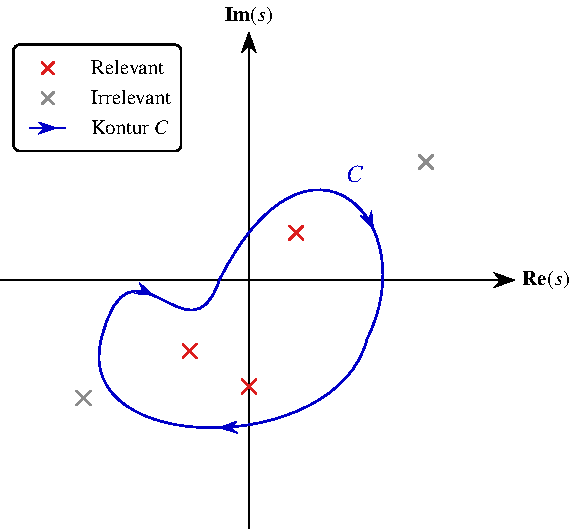
\includegraphics{papers/laplace/images/pol_auswahl.pdf}
    \caption{Auswahlregel des Residuensatzes:
    Nur die von der geschlossenen Kontur $C$ eingeschlossenen Polstellen
    (rot) liefern einen Beitrag $2\pi i \operatorname{Res}$ zum
    Konturintegral.
    Die Polstelle ausserhalb der Kontur (grau) ist für das Integral
    unsichtbar.}
    \label{laplace:fig:pol_auswahl}
\end{figure}
